\section{Modèle d'exécution fluxionnel}

\subsection{Fluxions}

Le modèle d'exécution fluxionnel a pour fonction de manipuler et d'invoquer des unités d'exécutions autonomes n'ayant pour paramètre d'entrée et de sortie que des flux, c'est à dire des séquences continues et infinies de données agrégées par messages.
Nous avons appelé ce type d'unité d'exécution autonome une fluxion.
C'est à dire une fonction, au sens de la programmation fonctionnelle, dépendant exclusivement de flux de données.
Elle est composée d'un nom unique, d'une fonction de traitement, et d'un contexte mémoire au moment de son exécution.

Les messages sont composés du nom de la fluxion destinataire et d'un corps, et acheminés par un système de messagerie.
% Ils représentent à la fois le signal d'invocation, et les données nécessaires à cette invocation.
Après avoir traité un message, la fluxion de traitement modifie son contexte local, puis termine son exécution en renvoyant un message sur son flux de sortie.
Chaque fluxion renvoie un message unique à destination d'une ou plusieurs fluxions.
Le contexte d'exécution de la fluxion de traitement est composé de l'ensemble des variables de mémoire dont dépend la fluxion pour pouvoir reprendre son traitement entre deux messages.

Les fluxions forment des chaînes de traitement liés par les flux.
L'ensemble de ces chaînes forme un graphe direct orienté.

\subsection{Système de messagerie}

Le système de messagerie est le cœur du modèle d'exécution fluxionnel.
Il a pour fonction, à la fois d'acheminer les flux de messages, et d'invoquer les fluxions.

Il est construit autour d'une file de messages, traités les uns après les autres par invocation de la fluxion destinataire.
L'utilisation d'une file de messages permet d'exécuter plusieurs chaînes de traitement parallèlement et équitablement, sans faire de différence dans l'ordonnancement entre messages locaux et messages provenant du réseau.
Le cycle de vie d'une application fluxionnelle est illustré figure \ref{fig:messagerie}.

\begin{figure}[h!]
  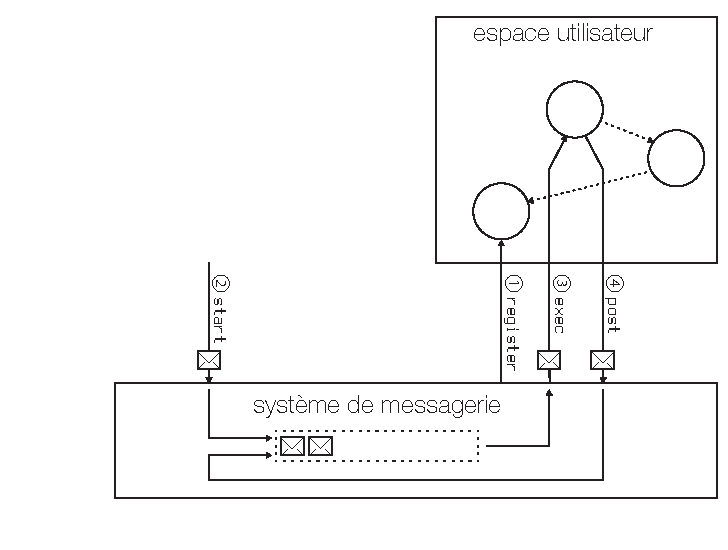
\includegraphics[width=0.5\textwidth]{schema-message.pdf}
  \caption{Schema du système de messagerie}
  \label{fig:messagerie}
\end{figure}

Chaque fluxion dois être enregistrée dans le système de messagerie.
Cet enregistrement associe une fonction de traitement à un nom, et un contexte d'exécution initial.
Le système de messagerie achemine les flux de messages en se basant sur les noms des fluxions.
C'est pourquoi il ne peut pas exister deux fluxions ayant le même nom.
% Lors de cet enregistrement, il est possible d'initialiser le contexte d'exécution.
L'enregistrement se fait à l'aide de la fonction \texttt{register(<nom>, <fn>, <contexte>)}, étape \circled{1} sur la figure \ref{fig:messagerie}.
% Une fluxion peut elle-même enregistrer d'autres fluxions dynamiquement.

Pour déclencher une chaîne de fluxions un premier message est envoyé à destination d'une fluxion par l'intermédiaire du système de messagerie, en utilisant la fonction \texttt{start(<msg>)}, étape \circled{2} sur le figure \ref{fig:messagerie}.
Cette fonction va placer un premier message dans la file.
Le système dépile ce message, et exécute la fonction de traitement destinataire, étape \circled{3} et \circled{4} sur le figure \ref{fig:messagerie}.
Le message résultat de cette exécution est alors empilé dans la file de message, étape \circled{5} et \circled{6} sur le figure \ref{fig:messagerie}.
Le système boucle alors sur les étapes \circled{3} à \circled{6} jusqu'à ce qu'il n'y plus de messages dans la file.

Les algorithmes \ref{alg:traitement} et \ref{alg:parcours} formalisent précisément le comportement du système de messagerie lors de l'appel de la fonction \texttt{start}.

\begin{algorithm}
\caption{Algorithme de la file de messages}
\label{alg:traitement}
\begin{algorithmic}
\Function{processMsg}{$msg$}
\For{$dest$ \textbf{in} $msg.dest$}
\State $fluxion \gets lookup(dest)$
\State $message \gets$ \Call{exec}{$fluxion, msg.body$} \Comment{\circled{4} \& \circled{5}}
\State \Call{enqueue}{$message$} \Comment{\circled{6}}
\EndFor
\EndFunction
\end{algorithmic}
\end{algorithm}

\begin{algorithm}
\caption{Algorithme de parcours de la file}
\label{alg:parcours}
\begin{algorithmic}
\Function{loopMessage}{\null}
\While{$msg$ \textbf{presents in} $msgQueue$}
\State $msg \gets$ \Call{dequeue}{\null} \Comment{\circled{3}}
\State \Call{ProcessMsg}{$msg$}
\EndWhile
\EndFunction
\end{algorithmic}
\end{algorithm}

\subsection{Interfaces externes}

% Les fluxions ne peuvent échanger de messages qu'avec les autres fluxions à l'intérieur du modèle d'exécution.
Afin de pouvoir interagir avec le monde extérieur, il faut définir des interfaces de bordures avec l'extérieur du système.
% Ces bordures sont capable à la fois d'interagir avec le système et avec l'extérieur.
% Ce lien d'interaction avec l'extérieur empêche les bordures d'être autonomes comme les fluxions.
Notre approche reposant principalement sur les architectures Web, l'interface visée est l'intégration des interfaces REST, qui engendre deux composants de bordures.

% Dans notre approche, il existe deux types d'interface de bordures pour le Web :

\begin{itemize}
	\item[\textbf{In}]
    permet de recevoir des connections clientes entrantes suivant le protocole REST.
    % C'est donc le premier maillon de la chaîne de traitement.
    Pour chaque connexion entrante, le composant \textbf{In} va transmettre au composant \textbf{Out} la connexion lui permettant de répondre au client Web, et un identifiant permettant d'associer messages et connexions.
    Il transmet ensuite l'identifiant à la première fluxion de la chaîne de traitement en appelant la fonction \texttt{start}.
	\item[\textbf{Out}]
    permet d'envoyer le résultat de la chaîne de traitement au client Web.
    Afin de recevoir les messages de la chaîne de traitement, le composant \textbf{Out} est enregistrée dans le système de messagerie.
    % C'est donc le dernier maillon de la chaîne de traitement.
\end{itemize}


Le schéma \ref{fig:schemaweb} présente les éléments d'un système Web fluxionnel et détaille les étapes d'acheminement d'un message par le système de messagerie.

\begin{figure}[h!]
	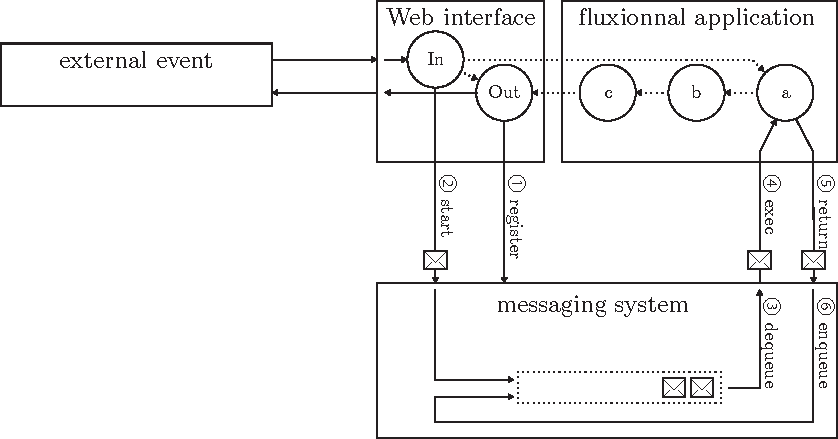
\includegraphics[width=0.5\textwidth]{schema-web.pdf}
	\caption{Schema d'un système fluxionnel avec une interface Web}
	\label{fig:schemaweb}
\end{figure}

% TODO paragraphe de transition

\subsection{Exemple de fluxion}

Afin d'illustrer le modèle d'exécution fluxionnel, nous présentons ici un exemple de son utilisation à travers un simple compteur de visite.

Ce service compte le nombre de connexions HTTP de chaque utilisateur et lui renvoie ce nombre dans la réponse.

\begin{figure}[h!]
  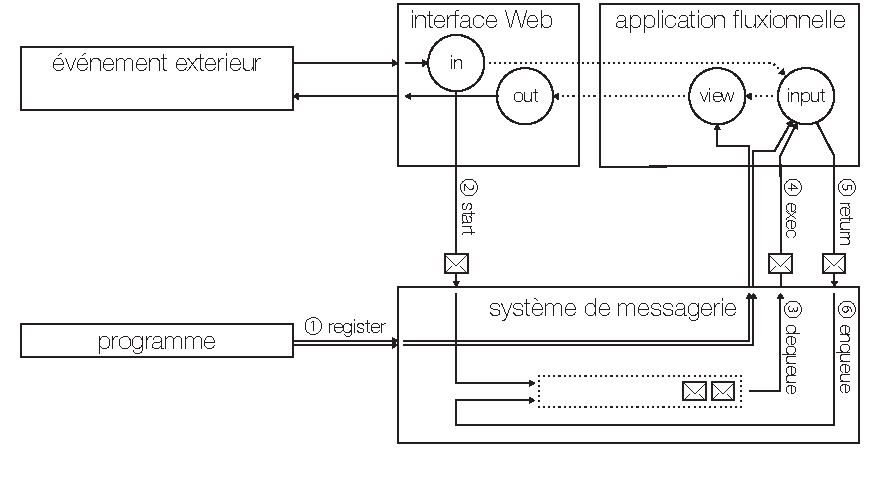
\includegraphics[width=0.5\textwidth]{schema-example.pdf}
  \caption{Schema de l'exemple d'un système fluxionnel avec une interface Web}
  \label{fig:example}
\end{figure}

La version initial du service pourrait représenter à l'extrait de code \ref{lst:classique}.

\begin{figure}
  \begin{code}
  var app = require('express')();

  var count = {};

  app.get('/:id', function reply(req, res){
    count[req.params.id] = count[req.params.id] + 1  || 1;
    var visits = count[req.params.id];
    var reply = req.params.id + '[' + visits + ']';
    res.send(reply);
  });

  port = 8080;
  app.listen(port);
  console.log("Listening port: "+port);
  \end{code}
  \caption{Service initial}
  \label{lst:classique}
\end{figure}

Dans ce code il faut distinguer 3 éléments.
La variable \texttt{count} est une mémoire persistante permettant de compter le nombre de visite pour chaque identifiant d'utilisateur distinc.
Elle sera donc transformée dans le notion de contexte d'exécution du système fluxionnel.
La fonction \texttt{reply} réalise le traitement fluxionnel type que l'on souahite réaliser.
Enfin les deux méthodes \texttt{get} et \texttt{send} permettent d'interagir avec le Web.

Ce programme minimal est transformé dans notre système selon les fluxions illustrés figure \ref{fig:fluxions}.

\begin{figure}[h!]
  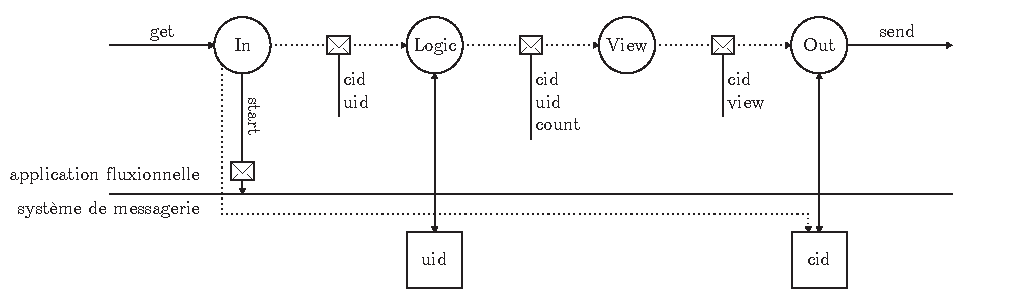
\includegraphics[width=0.5\textwidth]{flux.pdf}
  \caption{Suite de fluxion du compteur}
  \label{fig:fluxions}
\end{figure}

L'extrait de code \ref{lst:fluxionnel} décrit ce même service de comptage dans un pseudo code représentant le modèle d'exécution fluxionnel.

\begin{figure}
  \begin{code}
  var flx = require './lib/flx'
    , web = require './lib/external/web';

  fluxion input >> view
    this.uid[msg.uid] = this.uid[msg.uid] + 1 || 1;
    msg.count = this.uid[msg.uid];
    return msg;

  fluxion view >> output
    msg.view = msg.uid + "[" + msg.count + "]";
    msg.uid = undefined;
    msg.count = undefined;
    return msg;

  register input, {uid: {}}
  register view

  web.listen();
  \end{code}
  \caption{Code fluxionnel}
  \label{lst:fluxionnel}
\end{figure}

La code classique est bien plus concis que le code fluxionnel du fait de la segmentation et de l'encapsulation impliqué par le modèle fluxionnel.

Le service à été ségmenté comme suit :
\begin{itemize}
  \item[\circled{1}] Le point d'entrée \textbf{in} réagit à la connexion d'un client et démarre la chaîne de traitement en appelant \texttt{start}.
  Ce n'est pas une fluxion, il n'est pas enregistré dans le système de messagerie, et est lié à la machine recevant les connections entrantes.
  \item[\circled{4}] Le point de sortie \textbf{out} est enregistré dans le système comme une fluxion mais elle est liée à la machine recevant les connexions clientes afin de pouvoir y répondre.
  \item[\circled{2}] La fluxion \texttt{input} est la première à recevoir le message indiquant une connexion cliente. Son traitement consiste à incrémenter le compteur de l'utilisateur présent dans son scope, et à renseigner ce compteur dans le message, avant de le renvoyer à la fluxion suivante.
  Elle contient l'ensemble de la logique de ce simple service. Pour des services réels, on trouverais à sa place l'ensemble des fluxions contenant la logique du service organisé en une ou plusieurs chaîne de traitement.
  \item[\circled{3}] La fluxion \texttt{view} récupère le message, et met en forme la réponse que recevra l'utilisateur, et l'envoie à la fluxion de sortie.
\end{itemize}

Ce service manipule principalement deux informations sur lesquelles qu'il est important de détailler.
D'une part, les connections clientes sont partagé entre l'entrée et la sortie.
Pour chaque connexion, l'entrée passe directement à la sortie un couple <id, res>.
id représente simplement un identifiant permettant de retrouver res, il est envoyé à la fluxion input.
res est la structure permettant de répondre au client.
Ce mécanisme provoque un échange important de donnée entre le point d'entrée et le point de sortie, et implique de passer l'identifiant sur toute la chaîne de traitement, jusqu'à sa réception au point de sortie.

Les messages échangés contiennent principalement deux informations importantes : les identifiants d'utilisateurs, permettant d'incrémenter un compteur pour chaque utilisateur, et les identifiants de connexion, permettant de lier une suite de messages avec la structure contenant la connexion HTTP.
Le point d'entrée, et le point de sortie du système doivent rester sur la machine où la connexion a eu lieu pour avoir accès à l'interface réseau, tandis que les autre fluxions n'ont pas cette obligation, et peuvent être migré.


Cet identifiant de connexion est nécessaire au point de sortie pour associer le résultat reçu avec la connexion vers laquelle le renvoyer à l'utilisateur.
Nous passons cet identifiant pour ne pas alourdir les échanges de messages avec la structure contenant la connexion HTTP.

Ainsi, la fluxion de sortie reçois des messages provenant de deux fluxions : le point d'entrée




